\chapter{Mapping}
\label{ch:mapping}
An active magnetic shield relies on its coils to counteract field variations. A disturbance can only be compensated so well, as it can be approximated with the shield's coils. Therefore, an active shield will perform better if adapted to the magnetic environment, especially if the disturbances are high-order.

As part of the design process for an active shield for the n2EDM experiment a characterisation of the magnetic fields on its site was performed. To that purpose a magnetic field mapper was build---a tower equipped with magnetic field sensors.

First, a small-scale prototype of the mapper was tested during a mapping campaign in LPSC, Grenoble, France. It was then extended to full-scale and used for measurements on the site of the n2EDM experiment.




\section{The idea}
An essential input to the design of the n2EDM active magnetic shield was the scope of fields that would need to be compensated. There were a few strong magnetic sources in the vicinity of the site, some of them ramping on a daily basis. Taking a number of maps of the magnetic field was planned to characterise the magnetic environment.

Speed was valued more than precision. The shorter it would take to map the field in the whole area, the less it would be influenced by the varying external conditions. Also, the variety of the magnetic environment favoured taking multiple maps under different conditions, rather than few precise ones.
The implemented solution was a mobile tower equipped with magnetic field sensors at different heights. The position and orientation of the tower could be measured while it was moved around.

\begin{figure}
  \centering
  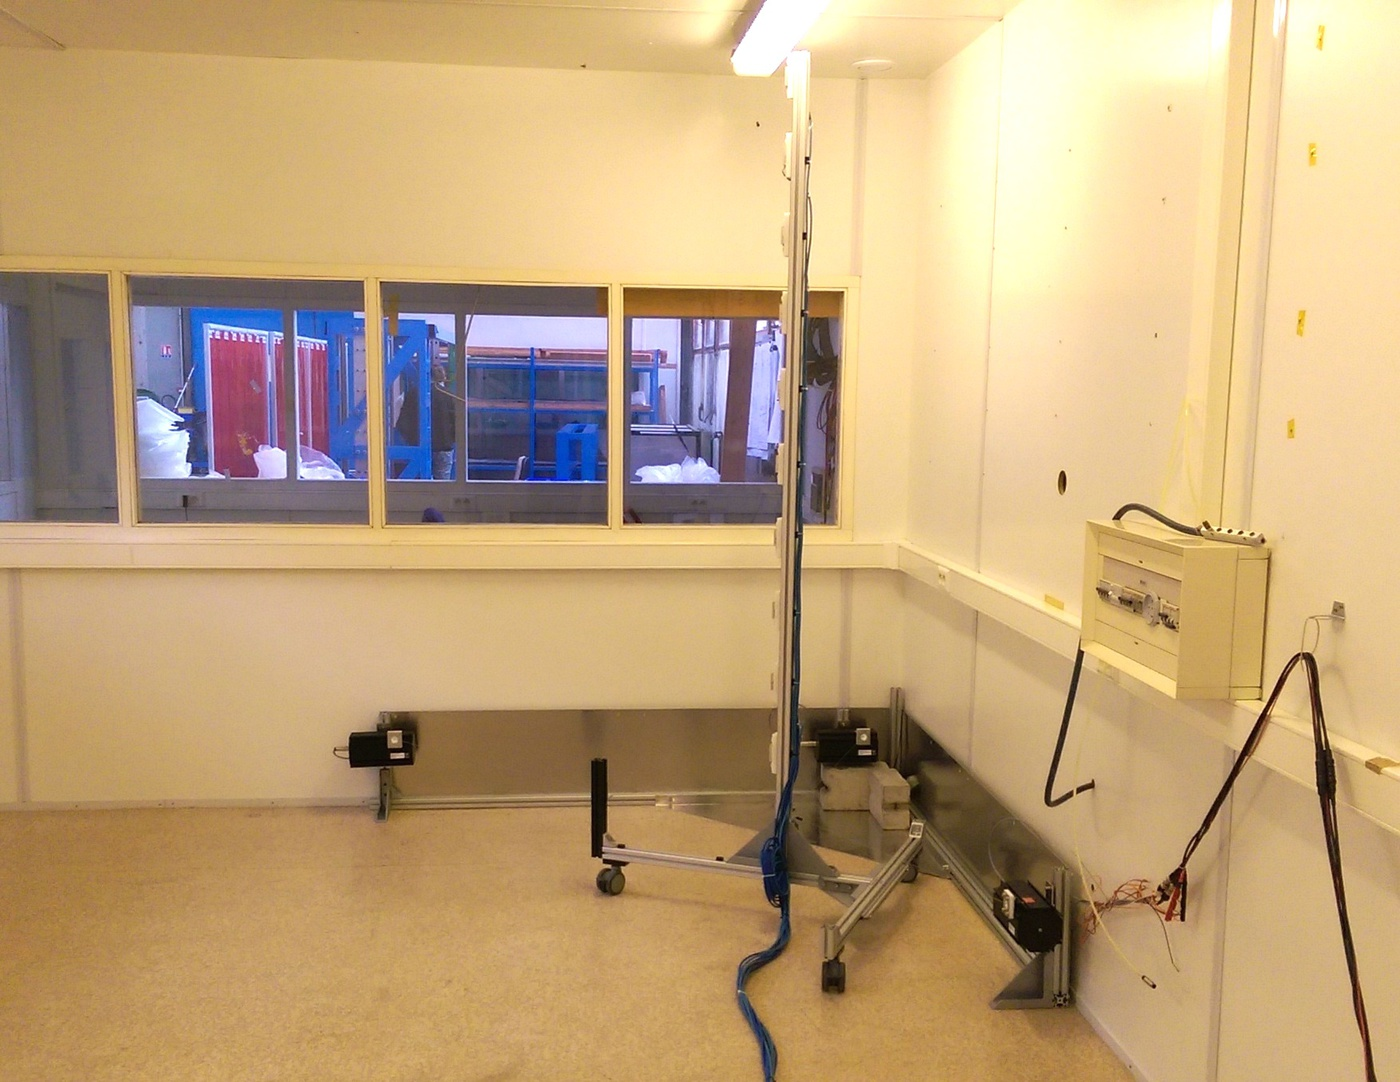
\includegraphics[width=\linewidth]{gfx/mapping/lpsc/setup_crop.jpg}
  \caption{The small-scale prototype of the magnetic field mapper. The mobile tower has ten fluxgate magnetometers attached to it. A bundle of readout cables is visible coming out of the tower. Behind it a rigid L-piece is visible, which has three string potentiometers mounted on it. A string is extended from each to the tower.}\label{fig:mapping_bastille_setup}
\end{figure}

% present tense - describing a picture
\marginpar{For maximal linearity string potentiometers are constructed in a way, that the wire is wound flat in one layer only.}
A small-scale prototype setup is pictured in Fig.\,\ref{fig:mapping_bastille_setup}. The tower
% is \SI{250}{\centi\metre} high and
has ten fluxgate magnetometers mounted on it. Behind the tower, in the corner, a rigid L-piece is visible. 
\marginpar{Other names for a string potentiometers include: cable-extension transducer, draw-wire sensor and string pot.}
It is carrying three black elements, string potentiometers, each with a thin wire coming out of it. The other end was attached to the tower. Inside a string potentiometer the wire is wound on a spring-loaded spool, the spool attached to a rotary potentiometer.
The potentiometer gives an analogue signal proportional to the extension of the wire. The combined information from the three sensors was used to determine the position and orientation of the tower.



\section{The principle of a string-potentiometer--based mapper}
For a known extension of a wire the set of points where the other end can be is a circle. The measurement of the position and orientation of the tower is, in fact, finding the intersections of those circles.
\marginpar{Other position determination methods include triangulation (measurement of angles between lines connecting a set of fixed points) and multilateration (measurement of the differences of distances between a set of fixed points).}
In general, the problem of determining the location based on the measurement of the distance to a set of fixed points is called \emph{trilateration}.

\begin{figure}
  \centering
  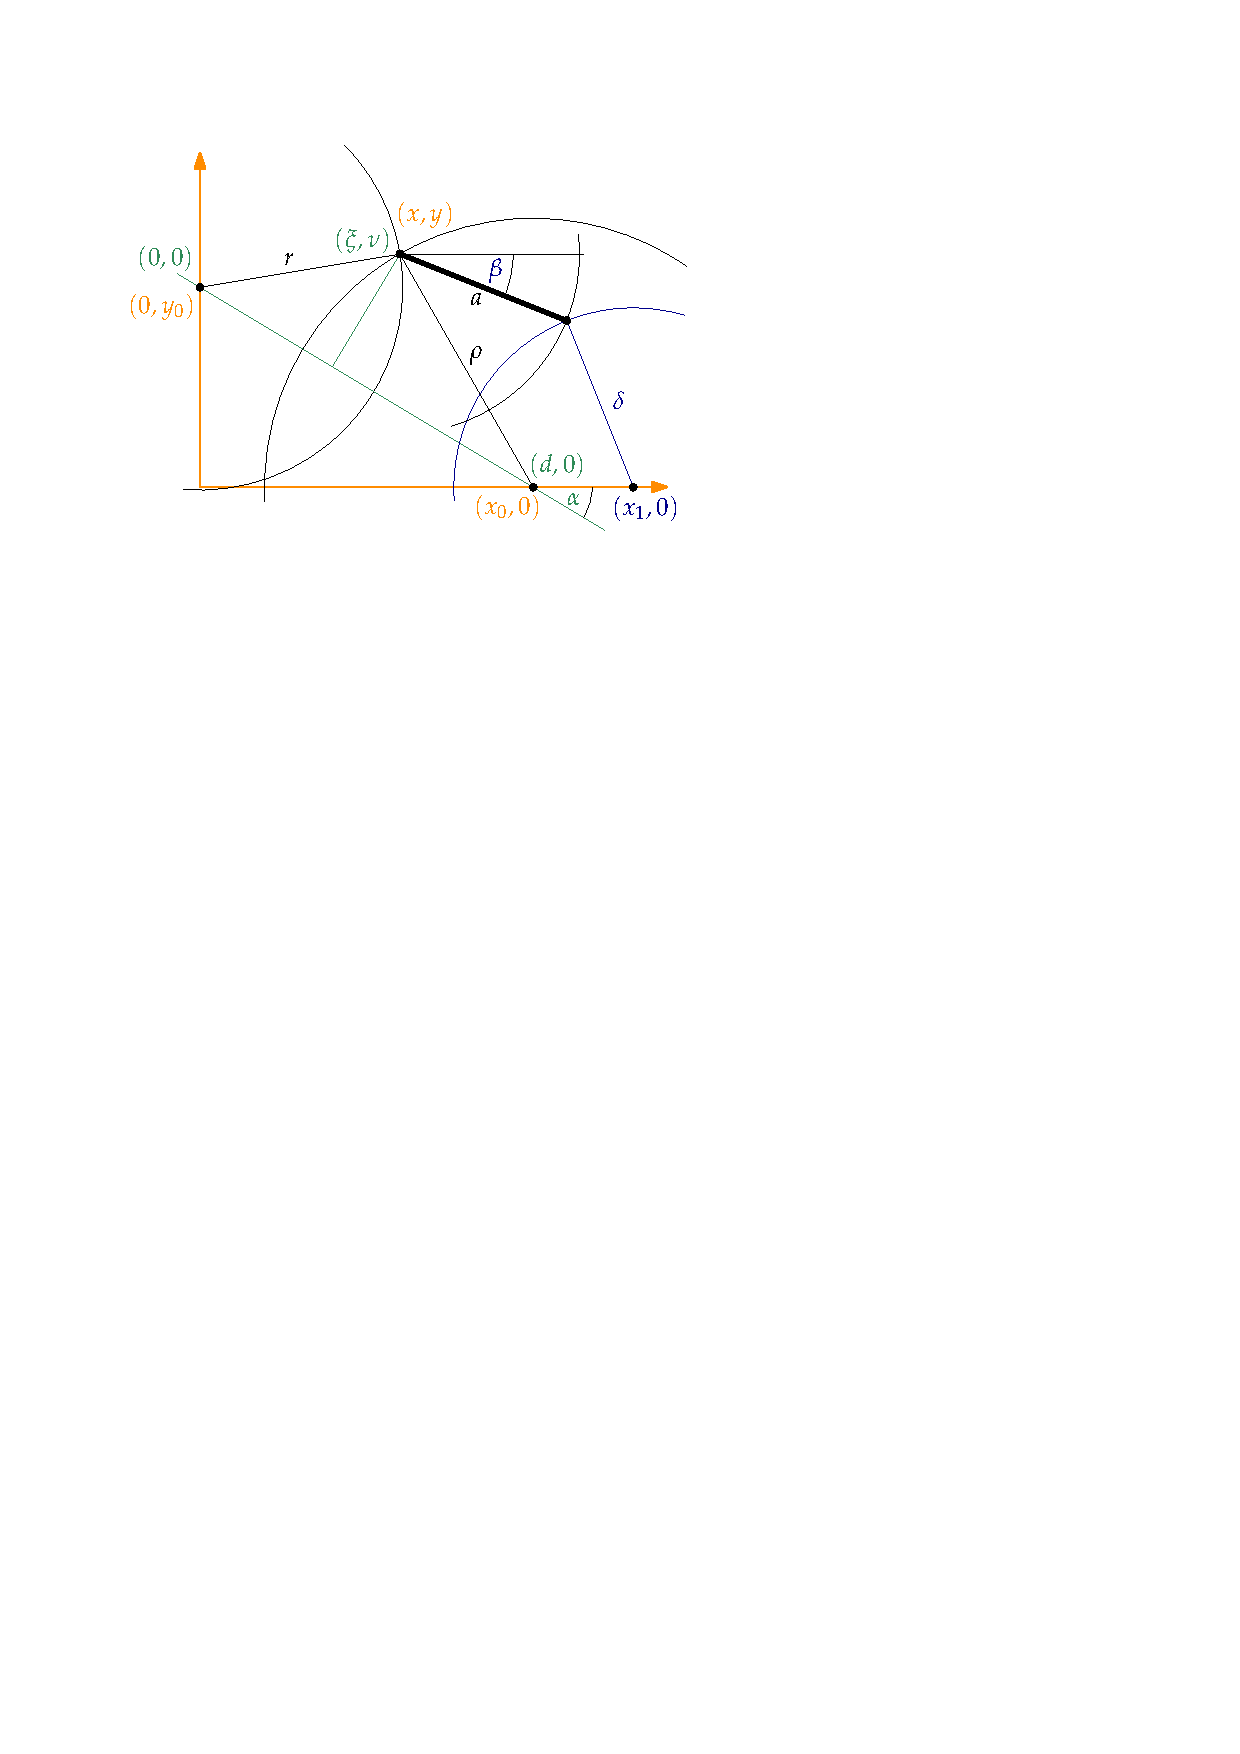
\includegraphics[width=0.7\linewidth]{gfx/mapping/geometry.pdf}
  \caption{The geometry of the mapper's position and orientation determination. The tower is depicted as a thick black line. In the orange coordinate system, the one of the ``L-piece'', the position of the centre of the tower is $(x,y)$. The positions of the string-potentiometers used to determine the tower's position are $(0, y_0)$ and $(x_0, 0)$ and the extensions of their wires: $r$ and $\rho$. Another, green, coordinate system is depicted, in which the position of one of the string-potentiometers is $(0,0)$ and the other $(d, 0)$. The position of the tower in this coordinate system is $(\xi, \nu)$. There is also a third string-potentiometer, its string, length $\delta$, attached to the tower on an arm of a length $a$.}\label{fig:mapping_geometry}
\end{figure}

The geometry is illustrated in Fig.\,\ref{fig:mapping_geometry}. The two string potentiometers used to determine the position are located is points $(x, y) = (0, y_0)$ and $(x_0, 0)$ (in the L-piece coordinate system, orange in the figure).
The wires of those two, their lengths $r$ and $\rho$, are connected to a single point $(x,y)$, which lied directly on the vertical beam holding the sensors. We will refer to the point as the centre, even though it is not necessarily the geometric centre of the tower. The centre lies on the intersection of the corresponding circles.
For the sake of simplicity, we first give the solution for the centre's position in the coordinate system depicted in green,
% \note{maybe use the A B and C names here already}
where the first string potentiometer is in $(0,0)$, the second in $(d, 0)$, with
\begin{equation}
  d = \sqrt{x_0^2 + y_0^2} \ ,
\end{equation}
and the tower's centre is in $(\xi, \nu)$. Then: 
\begin{align}
  \xi & = \frac{1}{2d} \left( d^2 - \rho^2 + r^2 \right) \\
  \nu & = \pm\ \frac{1}{2d} \sqrt{ (-d + \rho - r) (-d - \rho + r) (-d + \rho + r) (d + \rho + r) } \ .
\end{align}
There are two solutions, symmetric around the line connecting the centres of the circles. It was assumed that the tower never crossed that line.
The transformation of the solution to the ``L-piece'', orange, coordinate system is rotation by the angle 
\begin{equation}
  \alpha = \mathrm{ctan}\, \frac{y_0}{x_0} \ ,
\end{equation}
followed by a translation:
\begin{equation}
  \begin{pmatrix}
    x \\
    y
  \end{pmatrix}
  =
  \begin{pmatrix}
    \cos \alpha & -\sin \alpha \\
    \sin \alpha & \cos \alpha
  \end{pmatrix}
  \begin{pmatrix}
    \xi \\
    \nu
  \end{pmatrix}
  +
  \begin{pmatrix}
    0 \\
    y_0
  \end{pmatrix} \ .
\end{equation}
The orientation is determined with a use of the third potentiometer, its string attached to the tower at a distance $a$ from its centre. Then the position of the attachment point lies on the intersection of the circle centred at $(x,y)$ with radius $a$, and one centred at the potentiometer, radius equal to the measured extension of the wire $\delta$. In this case there are also two solutions, but ambiguity could be avoided by keeping the orientation of the tower approximately parallel to the $x$-axis.

In the prototype $x_0 = 0$. This had the consequence, that the precision of determining $x$ was poor when simultaneously $y$ was large and $x$ small. Then the two circles intersected at a very small angle. Due to measurement noise and uncertainty in calibration (the relationship between the analogue signal and the extension of the wires) sometimes the circles did not intersect at all. In those cases, the middle point of the shortest line connecting the circles was taken as the solution.

% in the same way, but with one circle centred in $(x,y)$, and the other at the 

% The problem of determining the orientation of the tower is, in fact, the same as the one of the position. The third string potentiometer, with the string attached to \note{there are two $d$s in the picture!} an arm of the tower (depicted in violet in Fig.\,\ref{fig:mapping_geometry}) of the length $a$. The end of the arm lies on the intersection of two circles: the one centred in the centre of the tower and radius $a$, and the one centred at the sensor end of the third potentiometer with the length equal to the wire extension.

% Technical notes.
% The precision of the position determination depends on the angle of the intersection of the two circles. In particular, if the centre lies on the line 

% If the string potentiometer used to determine the orientation is located at $(x_0 + a, 0)$, then the 



% \note{Comment on the sensitivity here. The solution is best conditioned, when the angle of the intersection of the circles is large. There is a problem, in particular, in the ``upper-left corner''.}



\section{LPSC campaign}
\label{sec:lpsc_campaign}
The small-scale prototype setup was used to perform a mapping of the magnetic field of two rooms in Laboratoire de Physique Subatomique \& Cosmologie (LPSC) in Grenoble, France. The campaign took place in the days 6.-10.03.2017, with the much appreciated help of Rémi Faure, Guillaume Pignol and Dominique Rebreyend. The rooms, referred to as \emph{Bastille} and \emph{Chalet}, were considered to host a magnetic-field-sensitive setup for ${}^{199}$Hg magnetometry. Of particular interest were the gradients, which cause an increase in the depolarisation rate of the mercury atoms~\cite{FertlThesis}.
\note{In that case the gradients should be below roughly \SI[per-mode=symbol]{10}{\nano\tesla\per\centi\metre}, but I don't know why. Ask someone?}
% In particular, gradients above roughly \SI[per-mode=symbol]{10}{\nano\tesla\per\centi\metre} 

\marginpar{The string potentiometers were equipped with custom made attachments, that allowed the string to come at an angle out of the device. The point where the strings bent was taken to be the middle of the circle in the geometry solution.}
A photograph of the mapping setup is shown in Fig.\,\ref{fig:mapping_bastille_setup}. The \SI{2.5}{\metre} high mobile tower was equipped with ten three-axis fluxgate magnetic field sensors (Stefan-Mayer FLC3--70, the same as used in the active magnetic field stabilisation system).
The stationary ``L-piece'' held three string potentiometers (Micro-Eplison WDS-15000-P115-SA-P with a \SI{15}{\metre} extension range).
The geometry parameters, as defined in Fig.\,\ref{fig:mapping_geometry}, were: $x_0 = 0$, $y_0 = \SI{1871}{\milli\metre}$, $x_1 = \SI{1756}{\milli\metre}$, $a = \SI{623}{\milli\metre}$. The string-potentiometer for the orientation measurement was in the point $(\SI{1756}{\milli\metre}, 0)$.

% Two of the strings were attached to a point where the vertical beam with the fluxgates is, the third (left on the picture) was attached to the black, short vertical profile on the tower.

% \marginpar{Technical details of the setup: fluxgates: Stefan-Mayer FLC3--70, ADC: aoethu, string potentiometers: Micro-Eplison WDS-15000-P115-SA-P, readout frequency: xxx}

\begin{figure}
  \centering
  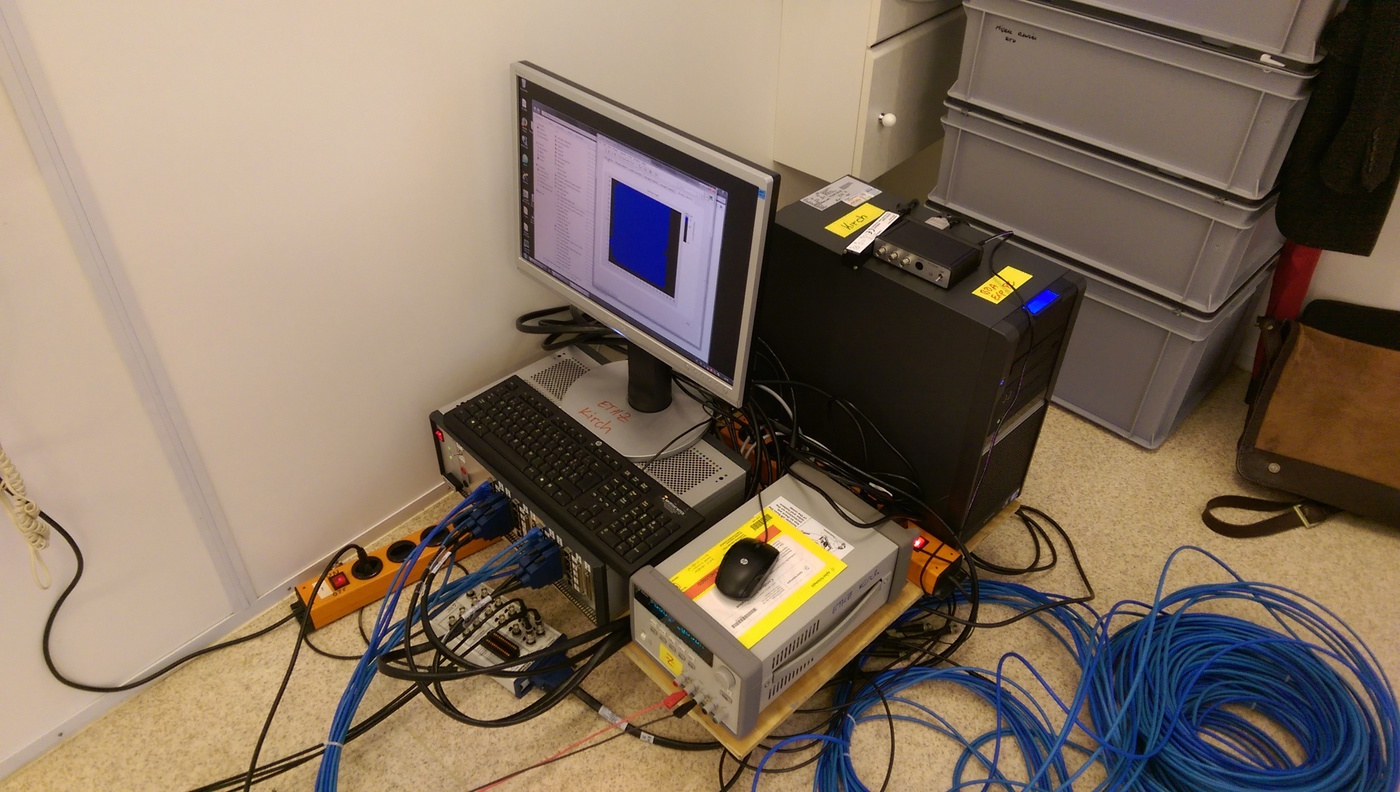
\includegraphics[width=\linewidth]{gfx/mapping/lpsc/daq.jpeg}
  \caption{The DAQ system used for the mapping campaign in LPSC\@: a power supply to put a constant voltage on the potentiometers (grey, lower corner); a custom-built crate for the fluxgates, which supplied them with power and conditioned the incoming signals (underneath the keyboard and the screen); a National Instruments PXI crate, which simultaneously digitised the analogue voltage signals from the fluxgates and the string-pots (not visible, behind the screen); and a PC computer with peripherals.}\label{fig:mapping_bastille_daq}
\end{figure}

The data acquisition system, pictured in Fig.\,\ref{fig:mapping_bastille_daq}, consisted of: a power supply that put a constant voltage (\SI{10}{\volt}) on the potentiometers; a custom-built crate for the fluxgates, which supplied them with power and conditioned the incoming signals; and a National Instruments PXI crate, which simultaneously digitised the analogue voltage signals from the fluxgates and the string-pots. The data were collected on a PC computer.

\begin{figure}
  \centering
  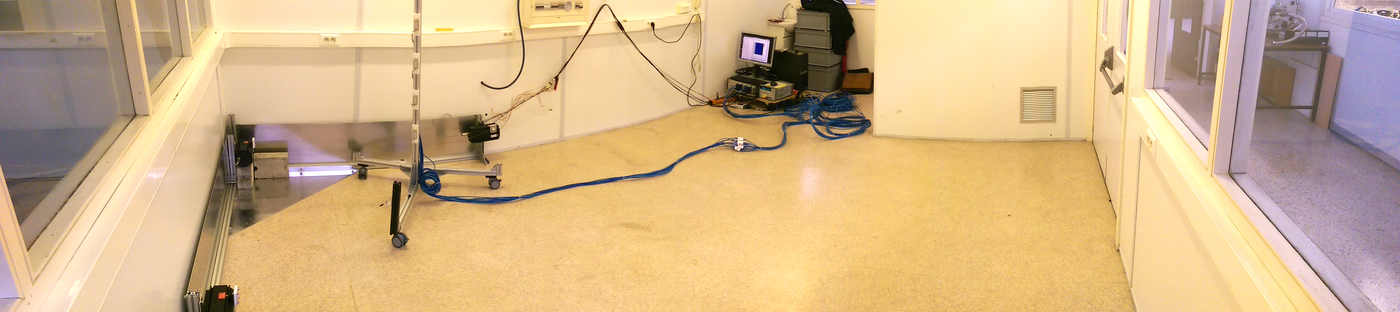
\includegraphics[width=\linewidth]{gfx/mapping/lpsc/bastille_panorama.jpeg}
  \caption{A panoramic view of the \emph{Bastille} room. To the left the ``L-piece'' and the mapping tower are visible. In the back there is the DAQ system and to the right a door with a long handle, which is also marked on the magnetic field maps.}\label{fig:mapping_bastille_panorama}
\end{figure}

A panoramic shot of the Bastille room is presented in Fig.\,\ref{fig:mapping_bastille_panorama}. The coordinate system is visible in the upper-left corner. To the right are the entrance door.
% In the middle, high on the wall, a power outlet box is visible.
% Behind the wall with the power outlet box there is a pump, which has been at some point removed.
The room was made out of wood. It stood inside a hall made of steel beams and sheets. 
% The room's wall with the power outlet on it was located close, less than 1 metre, to a steel wall of the hall.
The hall was equipped a gantry crane, several metres above the roof of the room.
% Directly on the roof there were air conditioning devices, standing about a metre above the roof on steel legs. The legs had rather large feet, possibly with a steel plate inside. 

\begin{figure}
  \centering
  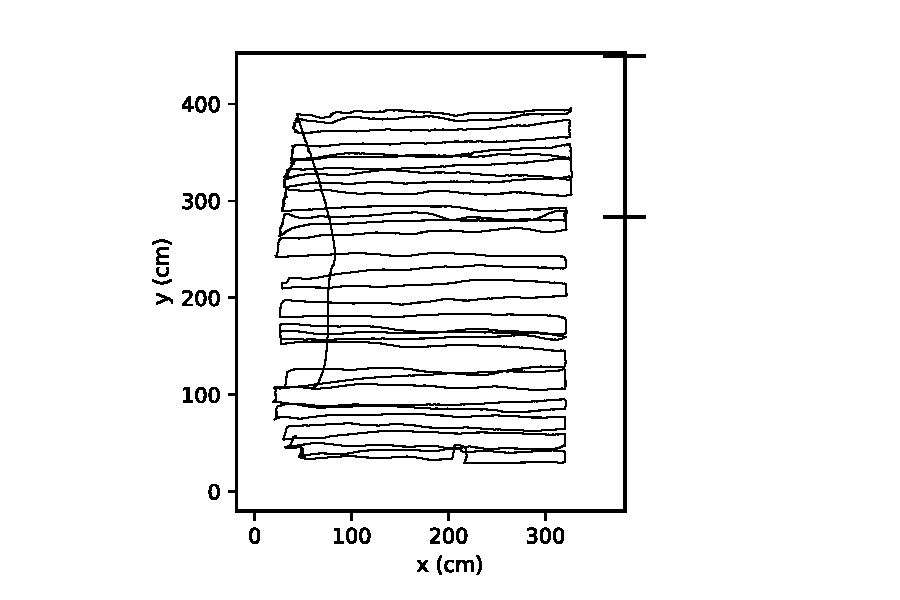
\includegraphics[width=0.5\linewidth]{gfx/mapping/lpsc/bastille_crane_away_rep_track_crop.pdf}
  \caption{The trace of the tower's centre in one of the maps. The outline of the room is marked. In the upper-right corner the location of the entrance door is marked. The ``L-piece'' was in the lower-left corner.}\label{fig:mapping_bastille_track}
\end{figure}

To collect a map the tower was moved around the room by one person, while another took care so that the readout cables did not get in the way.
\marginpar{The position was determined on-line. A display showed where the tower has already been.}
Care was taken to systematically scan the whole room and to maintain approximately the same orientation of the tower throughout the measurement. A track of one of the collected maps is depicted in Fig.\,\ref{fig:mapping_bastille_track}. Note, that the centre of the tower could only go to a certain distance to the walls, because of the size of the tower's cart.
%\note{maybe mention, that the position was calculated on-line, too}
% Part of the data analysis is performed on-line. In particular the voltage readout of the string pots is translated into their lengths which are used to determine the position and orientation of the tower. This is to provide feedback during the measurements, necessary to make sure that the whole room was scanned. 
The data, the position and orientation of the tower, as well as the magnetic field measurements, were down-sampled and registered at a \SI{50}{\hertz} rate.

\begin{figure}
  \centering
  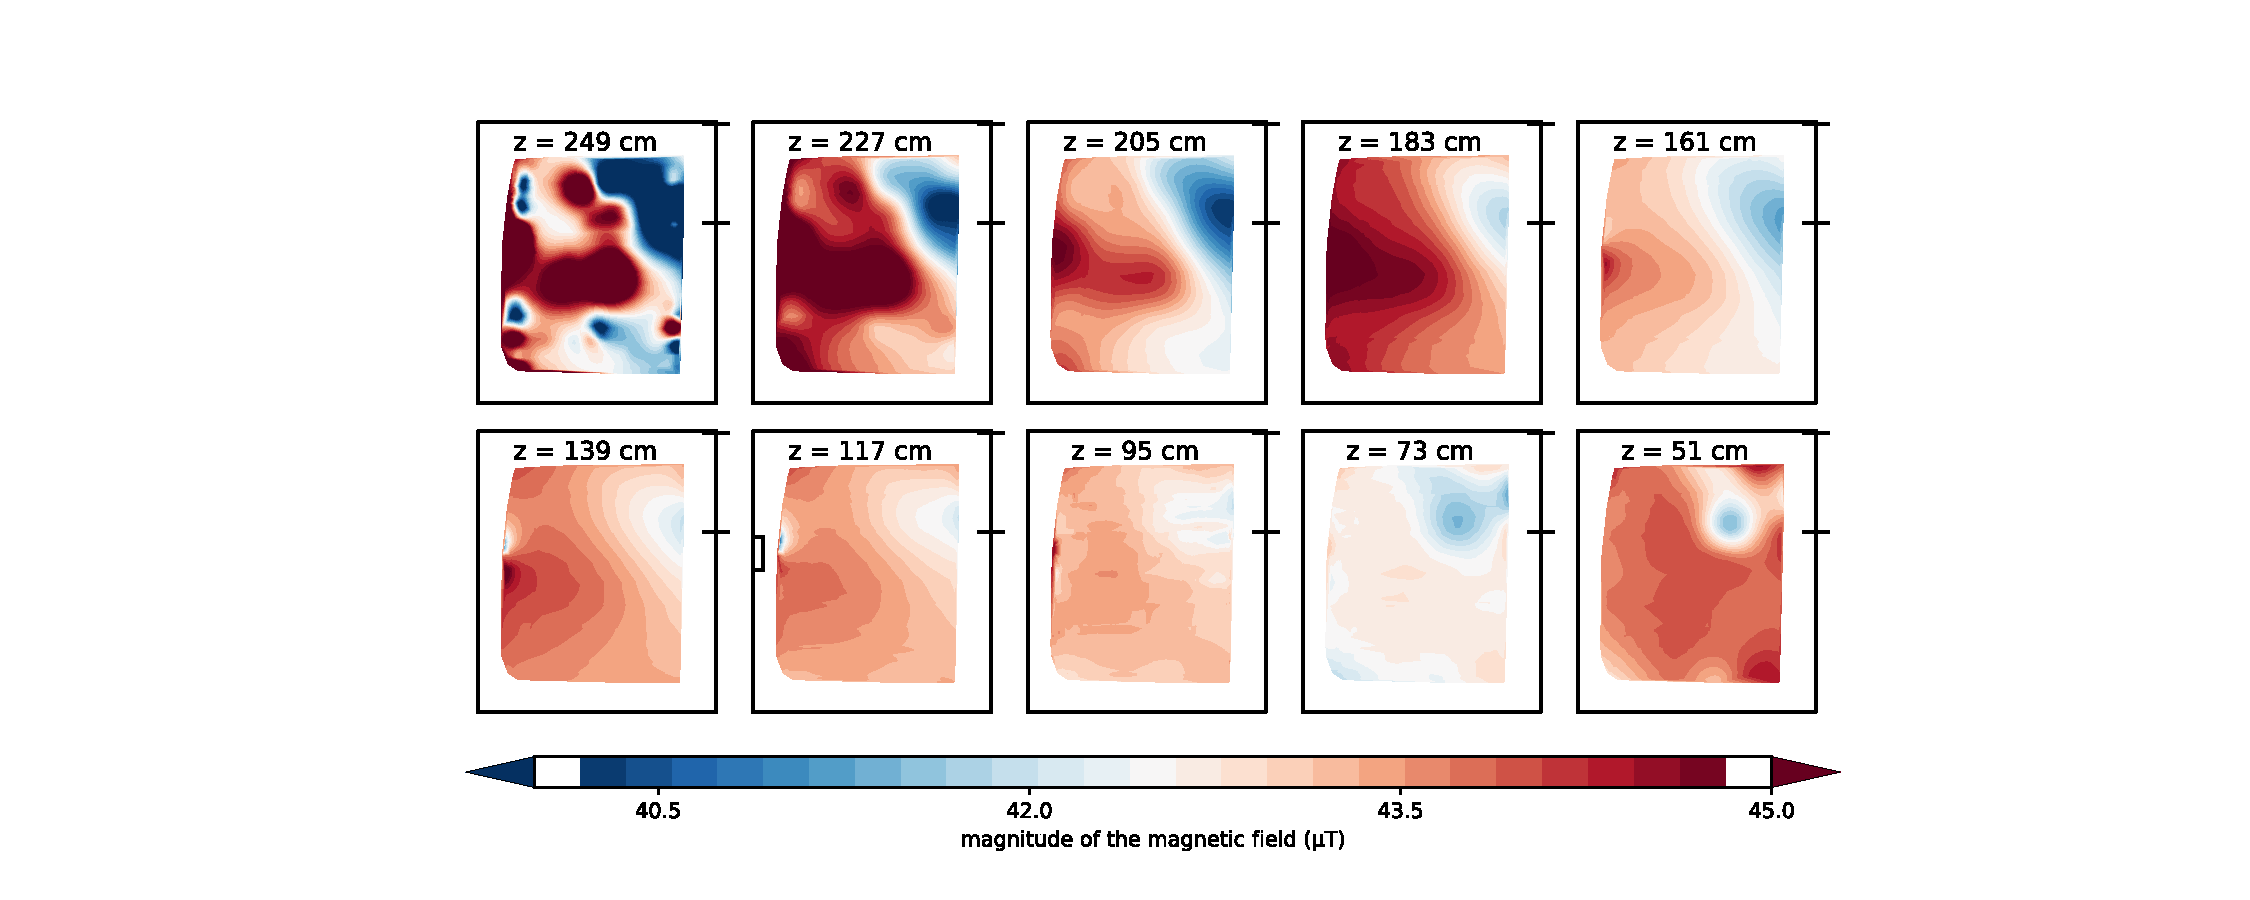
\includegraphics[width=\linewidth]{gfx/mapping/lpsc/bastille_crane_away_rep_magnitude_low_range_crop.pdf}
  \caption{The map of the magnitude of the magnetic field. Each tile depicts a horizontal plane, the field measured by one magnetic sensor. For each point, registered at \SI{50}{\hertz} rate, the magnitude is plotted; the colour in between the measurement points is linearly interpolated. On the ceiling there are small, strong sources of the magnetic field and the colour scale is saturated.}\label{fig:mapping_bastille_magnitude}
\end{figure}




\section{Data treatment}
\label{sec:mapping_lpsc_data_treatment}
A map of the magnetic field is plotted in Fig.\,\ref{fig:mapping_bastille_magnitude}. Horizontal slices (each a different sensor) of the magnitude of the magnetic field are shown, with the height of the slice above the floor indicated. Near the roof a number of localised sources are visible. It could be attributed to elements of an air-conditioning system mounted on the roof of the hut.

\begin{figure}
  \centering
  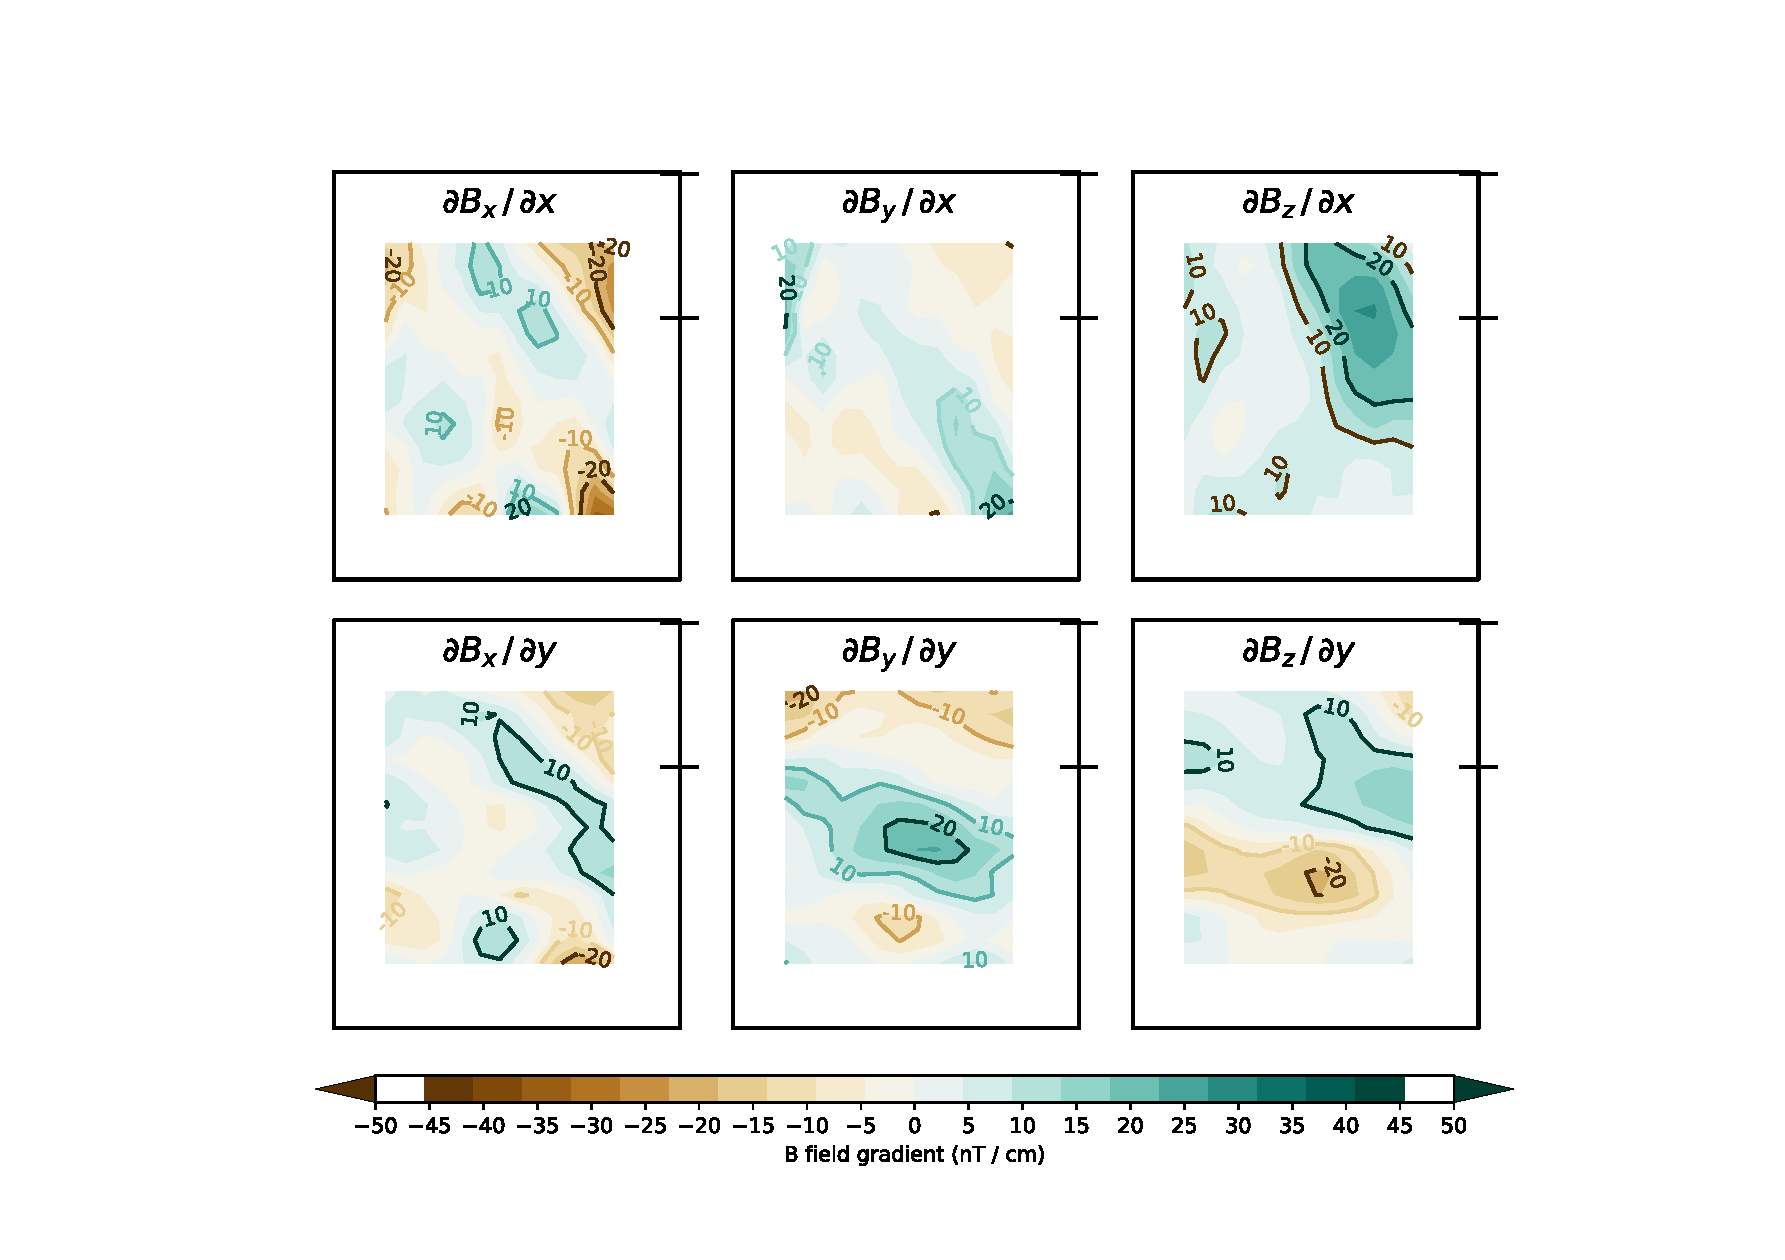
\includegraphics[width=\linewidth]{gfx/mapping/lpsc/bastille_crane_away_rep_gradient_205cm_crop.pdf}
  \caption{A map of the gradients in the \emph{Bastille} room \SI{205}{\centi\metre} above the floor. Only the ``horizontal'' gradients (with respect to $x$ and $y$) have been estimated. Estimating the one with respect to $z$ would require comparing measurements between different sensors, whose intrinsic offset would dominate the result.}\label{fig:mapping_bastille_gradient}
\end{figure}

The measured information was also used to estimate the gradients of the magnetic field. To this purpose the mapped area was divided into a $14 \times 14$ grid. In each bin the measurements were averaged.
Then the differences between the magnetic field components in the neighbouring pixels were taken, which, divided by the separation between the bins, were the estimates of the gradient.
% For example, the $\partial B_x / \partial x$ gradient was estimated by the difference between 
The map of the gradient \SI{205}{\centi\metre} above the floor is shown in Fig.\,\ref{fig:mapping_bastille_gradient}.
% Comment on the structures from the roof? On the left side, next to the power outlet box, large gradients above \SI[per-mode=symbol]{20}{\pico\tesla\per\centi\meter} are visible.
Only ``horizontal'' gradients were estimated, ones with respect to $x$ and $y$.
To estimate the vertical ones, with respect to $z$, would require to compare the measurements of different sensors. The sensors were specified to be only $\pm 1\% \pm \SI{0.5}{\micro\tesla}$ accurate, which in a roughly \SI{50}{\micro\tesla} field adds up to a microtelsa. With a \SI{22}{\centi\meter} separation between the sensors, the systematic effect on the gradient would be \SI[per-mode=symbol]{45}{\nano\tesla\per\centi\meter}. In the map gradients even below \SI[per-mode=symbol]{10}{\nano\tesla\per\centi\meter} are resolved.

\begin{figure}
  \centering
  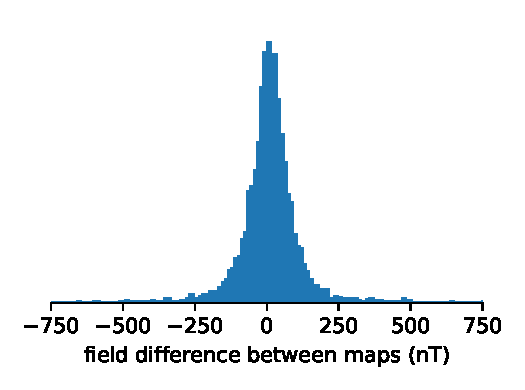
\includegraphics[width=0.49\linewidth]{gfx/mapping/lpsc/reproducibility_field.pdf}
  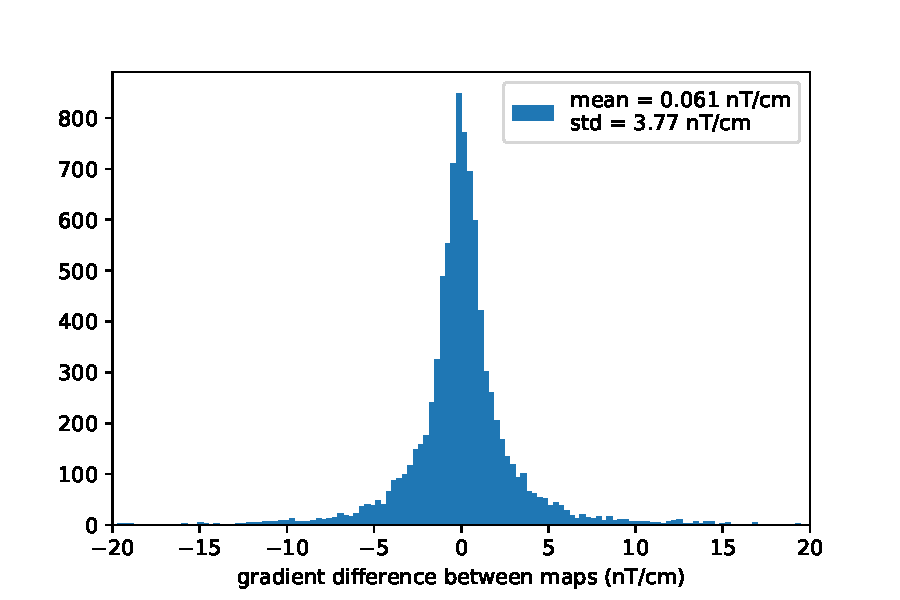
\includegraphics[width=0.49\linewidth]{gfx/mapping/lpsc/reproducibility_gradient.pdf}
  \caption{Left: Reproducibility of the field, a histogram of the difference in the measured field. One entry is a difference along either $x$, $y$ or $z$. The width of the distribution is \SI{138}{\nano\tesla}. Right: reproducibility of the gradient estimation. One entry is a ``horizontal'' gradient estimate, with respect to $x$ or $y$. The width of the distribution is \SI[per-mode=symbol]{3.8}{\nano\tesla\per\centi\metre}.}\label{fig:mapping_bastille_reproducibility}
\end{figure}

Binned data allowed also for direct comparison between maps. In order to estimate the reproducibility of the mapping process two maps were measured directly one after another. The maps were then, after binning, subtracted. The histogram of the differences is shown in Fig.\,\ref{fig:mapping_bastille_reproducibility}. The standard deviation of the distribution, a measure of the reproducibility, is \SI{138}{\nano\tesla}. The reproducibility of the gradient was estimated in the same way, yielding the standard deviation of \SI[per-mode=symbol]{3.8}{\nano\tesla\per\centi\metre}. This is better than a na\"{\i}ve estimate, which assumes that the value of the component of the field measured in one, $\approx \SI{25}{\centi\metre}$ large bin has a \SI{138}{\micro\tesla} uncorrelated error bar associated with it:
\begin{equation}
  \frac{\SI{138}{\nano\tesla} \, \sqrt{2}}{\SI{25}{\centi\meter}} = \SI[per-mode=symbol]{8}{\nano\tesla\per\centi\meter} \ .
\end{equation}
The reason is, that the for the absolute field estimate to be reproducible the system needs to be stable on a long time-scale, from one map to another. For the gradient of the field to be reproducible, the system needs to be stable only from one bin to the next.

\begin{figure}
  \centering
  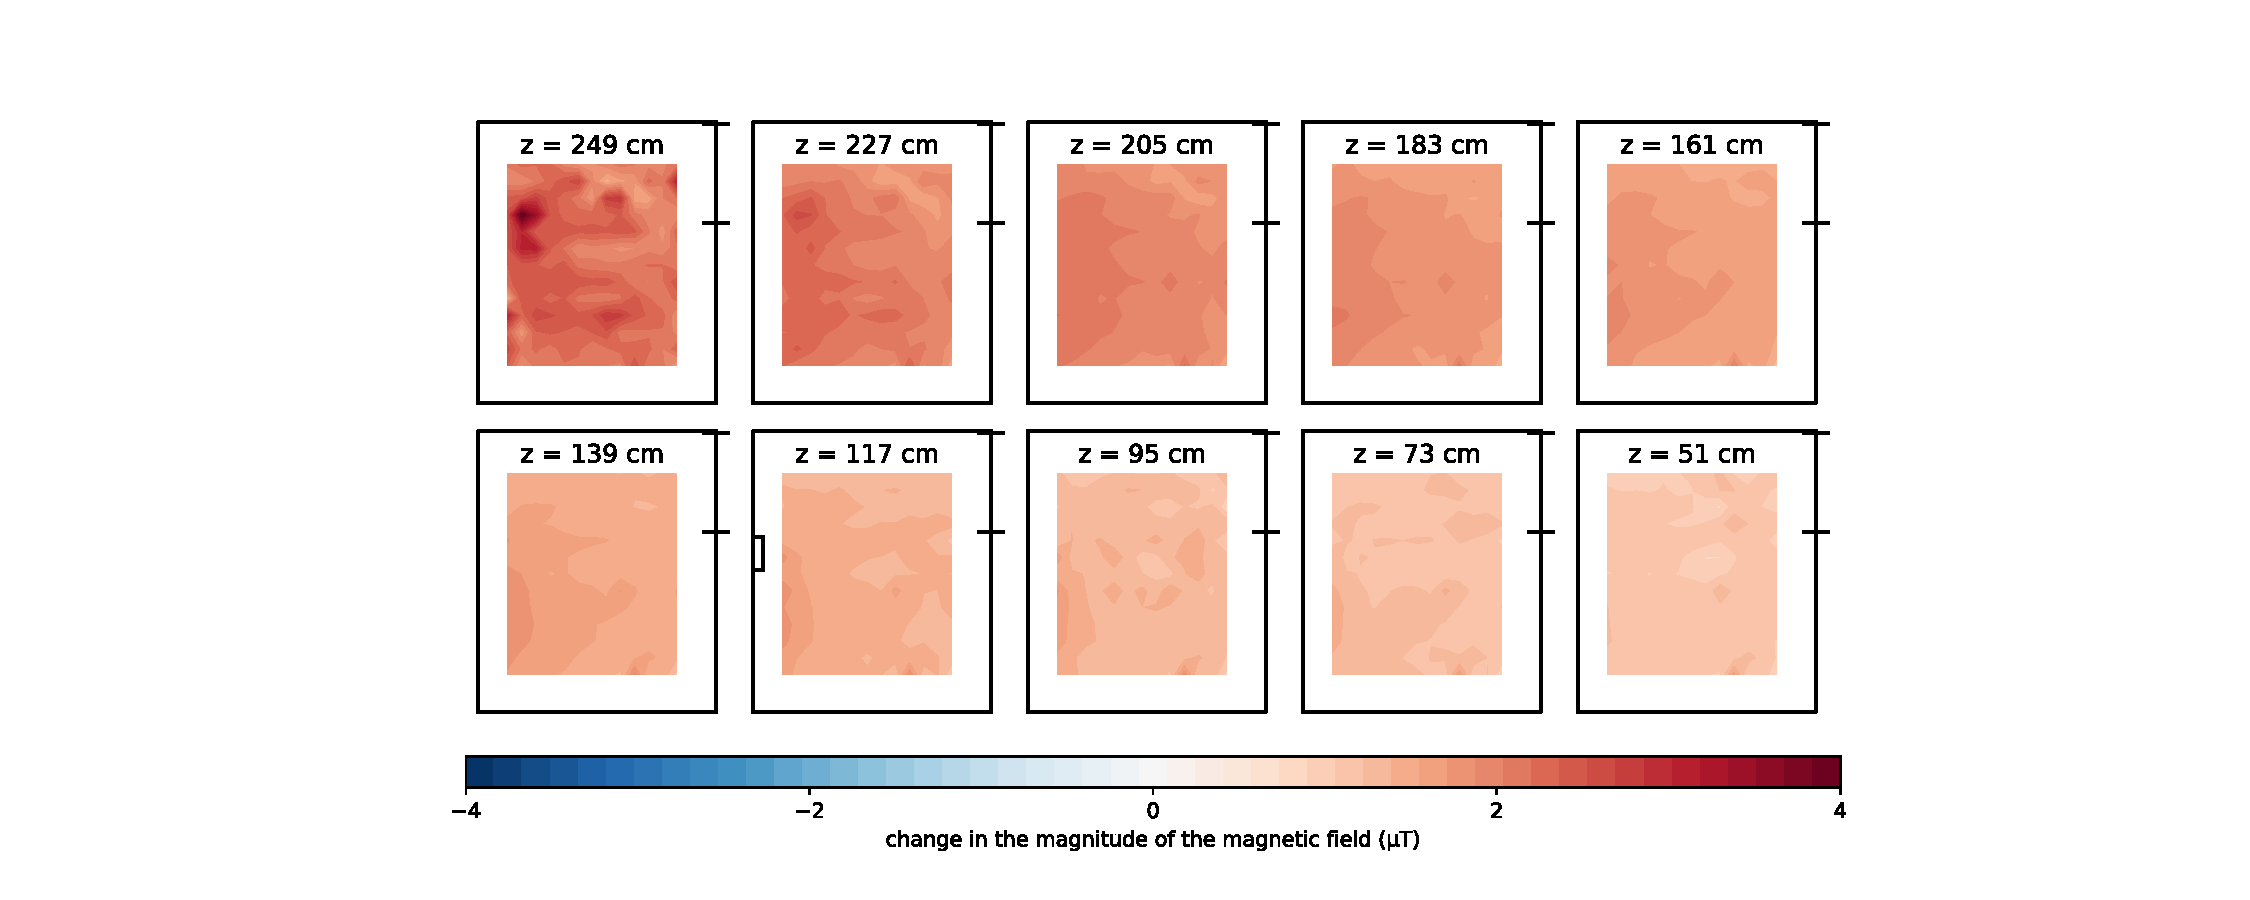
\includegraphics[width=\linewidth]{gfx/mapping/lpsc/bastille_crane_change_magnitude_crop.pdf}
  \caption{A map of the magnetic field of a gantry crane in the hall where the Bastille room is located. The magnitude of the field difference between two maps is plotted: one with the crane directly above the hut, and one with it moved far away.}\label{fig:mapping_bastille_crane_change}
\end{figure}

Also two maps taken in different conditions can be compared. Near the roof of the hall where the Bzastille hut was located there was a large gantry crane. In order to estimate the change in the magnetic field it inflicted when moving two maps were taken: one with the crane in the far end of the hall and another with the crane directly above the hut. The maps were binned. Their difference is plotted in Fig.\,\ref{fig:mapping_bastille_crane_change}. The magnetic field produced by the crane in the room is about \SI{1}{\micro\tesla} strong half a metre above the floor, furthest from the crane, and rises to \SI{3}{\micro\tesla} at the room's roof.
% Horizontally the change is homogeneous on a \ldots level.
% \mnote{A more detailed analysis of this map, maybe? But not really necessary.}


% \begin{figure}
%   \centering
%   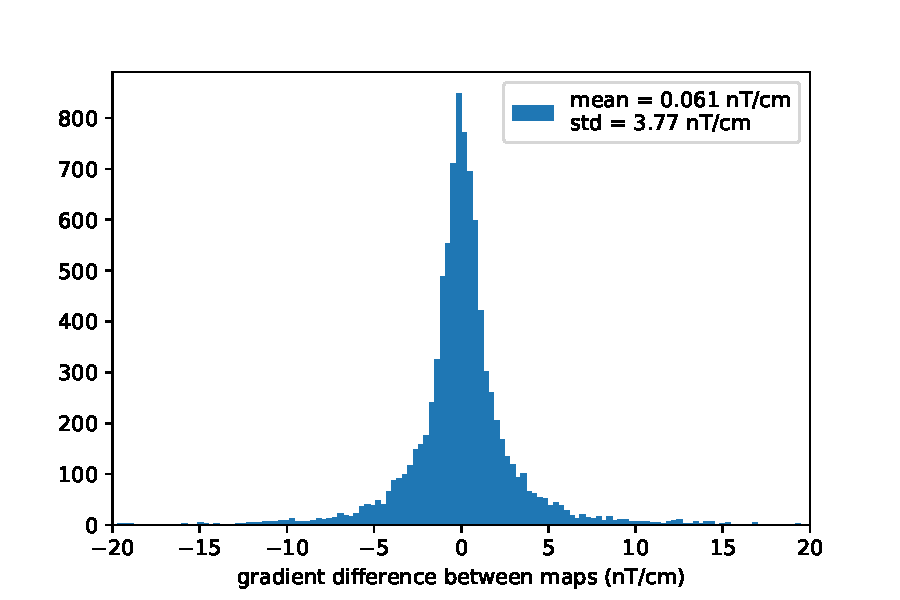
\includegraphics[width=0.8\linewidth]{gfx/mapping/lpsc/reproducibility_gradient.pdf}
%   \caption{\ldots}
%   \label{fig:mapping_bastille_magnitude}
% \end{figure}

The campaign at LPSC first of all resulted in a detailed magnetic characterisation of the Bastille and Chalet rooms, considered to be magnetometry laboratories. (The maps of the Chalet rooms can be found in App.\,\ref{ch:chalet_appendix}.) Secondly, it demonstrated the capabilities of the magnetic field mapping with a mobile tower, whose position and orientation is determined with string potentiometers. The prototype was later enlarged in preparation for a mapping of a much larger volume, one where the n2EDM experiment was to be built.




\section{PSI Area South campaign}
The mapping of the Area South in the UCN hall at PSI, the location of the nEDM and n2EDM experiments, took place in the days 19.12.2017--12.01.2018. In that time the area was empty; the nEDM apparatus had already been disassembled and a reinforced concrete foundation for the n2EDM experiment had been laid.
% After the n2EDM apparatus would be set up it would occupy the area and no magnetic mapping will be possible.
The goal of the mapping campaign was to characterise the magnetic field environment, in particular the different fields created by nearby magnets.
The information would provide the information necessary to design an active system, that would efficiently compensate for those fields.
The mapping campaign was a joint venture with Solange Emmenegger and Jochen Krempel.
% \marginpar{The mapping took place in the days 18--22.12.2017 and 2--12.01.2017.}
% Acknowledge that it is a joint work with Solange Emmenegger and Jochen Krempel.

\begin{figure}
  \centering
  \includegraphics[width=\linewidth]{gfx/mapping/PSI_mapping_photos/image_nedm-constructioncam2_2018-01-12_13-04-00.jpg}
  \caption{The Area South in the UCN hall at PSI\@. The brown square is the foundation for the n2EDM apparatus, covered with carton. }\label{fig:mapping_photo}
\end{figure}

% First say about the area - how large, refer to a picture.
\marginpar{The total weight of the n2EDM shield is 47 tons.}
The prototype mapper used in the LPSC campaign was extended to its full-scale. The Area South, pictured in Fig.\,\ref{fig:mapping_photo}, is about $10 \times \SI{12}{\metre}$ large.
The $5.2 \times 5.2 \times \SI{4.8}{\metre}$ magnetic shield of n2EDM would reach up to almost \SI{7}{\metre}. In the full-scale setup the parameters, defined as in Fig.\,\ref{fig:mapping_geometry}, were:
$x_0 = 0$, $y_0 = \SI{3814}{\milli\metre}$, $x_1 = \SI{3673}{\milli\metre}$, $a = \SI{965}{\milli\metre}$. The tower was \SI{8}{\metre} high.
\marginpar{The tower was built out of aluminum trusses, typically used for stages.}
An additional magnetic field sensor directly above the floor was added. Other than that, no changes from the prototype were made. The string potentiometers, the magnetic field sensors and the data acquisition system remained the same.

% The mapper used in the LPSC campaign needed to be enlarged, so that it could map the whole volume in the Area South.
% The volume to map was much larger then it was the case in the LPSC campaign. and the device needed to be enlarged. The `L-piece' was enlarged to \ldots. The tower was \SI{8}{\metre} high. An additional sensor was added directly above the floor. The other elements, string potentiometers, magnetic field sensors and DAQ, remained the same. \note{get the geometry}
% Then say what kind of mapper was necessary to map that. Most of the hardware kept, just made larger.
% The Area South is pictured in Fig.\,\ref{fig:mapping_photo}. It is roughly \note{GET THE SIZE} in size. The n2EDM magnetically shielded room, $5 \times 5 \times \SI{5}{\metre}$ large itself, ends \note{the height}.

\begin{figure}
  \centering
  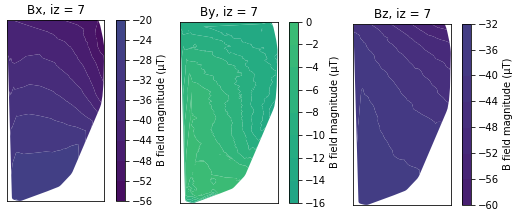
\includegraphics[width=\linewidth]{gfx/mapping/nSnCobCom.png}
  \caption{A map of the magnetic field in one plane, height around \note{HEIGHT} above the floor. \note{Get a plot from Solange with the outline of the hall marked, or make one myself. The trace of the tower should be marked there, too!}}\label{fig:mapping_photo}
\end{figure}

% Now about the magnets - COMET, SULTAN and COBRA. SULTAN daily ramps, COBRA and COMET just one ramp. Many maps and then combination thereof.
There were three strong magnets close to the area: COMET, SULTAN and COBRA\@. COMET is a medical cyclotron located several meters into the concrete biological shielding on the far-side wall in Fig.\,\ref{fig:mapping_photo}. Its field, very inhomogeneous due to the vicinity of the source, was around \SIrange[range-phrase=--,range-units=single]{10}{50}{\micro\tesla} strong. COMET is very rarely turned off. Fortunately, during the mapping campaign there was scheduled power-cut, for which the cyclotron was ramped down. SULTAN is a superconducting magnet for material research, located around \SI{15}{\metre} away from the site. It ramps daily, creating a roughly \SI{50}{\micro\tesla} field in the area. COBRA is a magnet located in a neighbouring experimental hall. The strength of its field is around \SI{5}{\micro\tesla}.

In total 25 maps were taken with various combinations of the states of the magnets. The maps are summarised in Tab.\,\ref{tab:psi_mapping_maps}.
As of April 2018 the analysis of this maps in ongoing~\cite{EmmeneggerThesis}.
The procedure of binning and subtracting the maps (Sec.\,\ref{sec:mapping_lpsc_data_treatment}) will allow the field of each of the three magnets to be estimated. The measurements will be an important input to the design of the n2EDM active magnetic shield. They will help to decide what coils should be built. It could even be possible to design coils dedicated for a particular high-order disturbance, like COMET\@.

\begin{table}
  \centering
  \begin{tabular}{ccrrr}
    date        &  time   &  SULTAN   &  COBRA  &  COMET \\ \midrule
    19.12.2017  &  17:32  &  100\%    &  100\%  &  100\%  \\
    19.12.2017  &  17:55  &  0\%      &  100\%  &  100\%  \\
    21.12.2017  &  10:04  &  95\%     &  100\%  &  100\%  \\
    21.12.2017  &  10:19  &  ramping  &  100\%  &  100\%  \\
    21.12.2017  &  11:53  &  90\%     &  100\%  &  100\%  \\
    21.12.2017  &  11:56  &  90\%     &  100\%  &  100\%  \\
    21.12.2017  &  13:38  &  20\%     &  100\%  &  100\%  \\
    21.12.2017  &  14:23  &  20\%     &  100\%  &  100\%  \\
    21.12.2017  &  16:36  &  20\%     &  100\%  &  50\%   \\
    21.12.2017  &  16:47  &  ramping  &  100\%  &  50\%   \\
    21.12.2017  &  17:35  &  0\%      &  100\%  &  100\%  \\
    22.12.2017  &  10:55  &  0\%      &  100\%  &  100\%  \\
    04.01.2018  &  15:41  &  0\%      &  0\%    &  100\%  \\
    04.01.2018  &  17:01  &  0\%      &  0\%    &  100\%  \\
    04.01.2018  &  17:17  &  0\%      &  0\%    &  100\%  \\
    05.01.2018  &  14:59  &  0\%      &  0\%    &  0\%    \\
    05.01.2018  &  15:22  &  0\%      &  0\%    &  0\%    \\
    05.01.2018  &  16:12  &  0\%      &  0\%    &  0\%    \\
    05.01.2018  &  16:41  &  0\%      &  0\%    &  0\%    \\
    05.01.2018  &  20:26  &  0\%      &  0\%    &  0\%    \\
    09.01.2018  &  10:55  &  0\%      &  0\%    &  100\%  \\
    09.01.2018  &  11:30  &  0\%      &  0\%    &  100\%  \\
    12.01.2018  &  10:31  &  0\%      &  0\%    &  100\%  \\
    12.01.2018  &  10:55  &  0\%      &  0\%    &  100\%  \\
    12.01.2018  &  14:11  &  0\%      &  0\%    &  100\%  \\
  \end{tabular}
  \caption{List of the maps taken. The status of the magnets is given for each in approximate percentage of the maximum field measured during the campaign.}\label{tab:psi_mapping_maps}
\end{table}




\section{Conclusion}
Active shielding greatly improved magnetic field stability at the nEDM experiment at PSI\@. The design of a shield for its successor, n2EDM, proved to be challenging due to tight spatial constraints.

A new method of magnetic field coil design targeted exactly the problem of spatial constraints. In the design process the coils are constrained to a predefined grid, which can be defined to fulfil the constraints. The coils also have a very large fiducial volume, which meant they could be fitted tightly around the apparatus.

A prototype of a grid-based active shield demonstrated the unprecedentedly large fiducial volume. Thereby it constructively showed, that an active magnetic shield for the n2EDM experiment can be built.

The maps of the magnetic field at the site of n2EDM would provide a crucial input to the design of the coils of the active shield. The design could be done fully within the framework of the new coil design method.

The developments of this work laid the foundation for an active magnetic shield for the n2EDM experiment, which would reduce the tens-of-microteslas variations down to just a few.